\chapter{Methodology and Experiments Setup}\label{cap:methodology}
This chapter presents the benchmark minimization problems used in our experiments and the experimental methodology, including the test environment, evaluation metrics and experimental setup.

\section{Benchmark Functions}
We use the benchmark functions proposed by Tang \emph{et al.} in 2010 \cite{CEC:Tang2010}, that are appropriate to optimization of high dimensionality. There are 20 functions, which have different degrees of separability and are divided in four types of high-dimensional problems \cite{CEC:Tang2010}: (i) Separable functions; (ii) Partially-separable functions, in which a small number of variables are dependent while all the remaining ones are independent; (iii) Partially-separable functions that consist of multiple independent subcomponents, each of which is $m$-non-separable; and (iv) Fully-nonseparable functions.

The benchmark functions use the following functions as basic functions \cite{CEC:Tang2010}:
\begin{itemize}
  \item The Sphere Function: The Sphere function (observe Figure \ref{fig:CEC_Sphere}) is defined according to Equation (\ref{eq:CEC_Sphere}).
    \begin{equation}\label{eq:CEC_Sphere}
    F_{Sphere}(\vec{x}) = \sum_{i=1}^{D}x_i^2,
    \end{equation}
    in which $D$ is the number of dimensions and $\vec{x} = (x_1, x_2, \ldots, x_D)$ is a $D$-dimensional row vector (i.e., a $1 \times D$ matrix). The Sphere function is very simple and is manly used for optimization.
    \begin{figure}[!h]
    \centering
    \subfigure[]{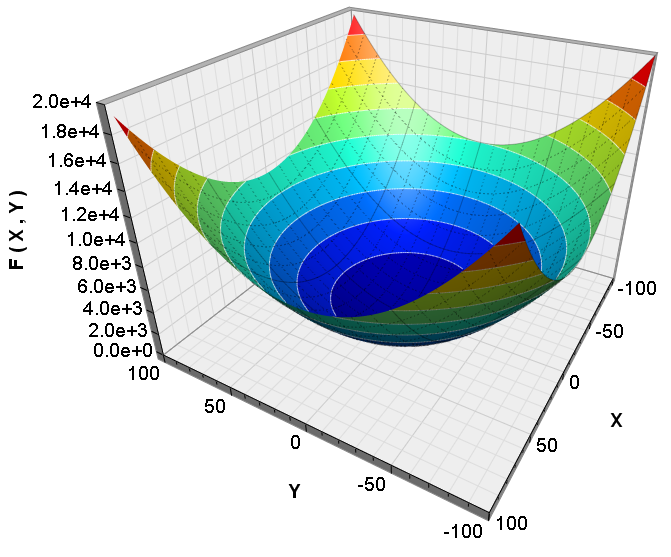
\includegraphics[scale=0.35]{graphics/Sphere_3d.png}\label{fig:CEC_Sphere_3d}}
    \hspace{1mm}
    \subfigure[]{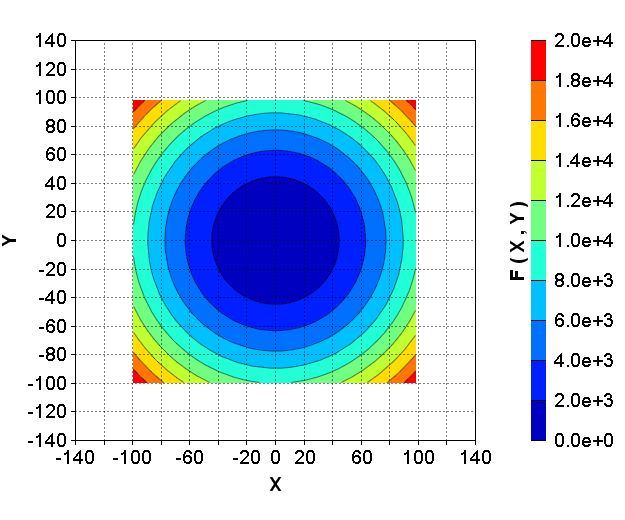
\includegraphics[scale=0.35]{graphics/Sphere_cont.png}\label{fig:CEC_Sphere_cont}}
    \caption{Illustration of Sphere function: (a) Surface and (b) Contour.}
    \label{fig:CEC_Sphere}
    \end{figure}

  \item The Rotated Elliptic Function: the original Elliptic Function is separable, and is defined according to Equation (\ref{eq:CEC_Elliptic}).
    \begin{equation}\label{eq:CEC_Elliptic}
    F_{Elliptic}(\vec{x}) = \sum_{i=1}^{D}(10^6)^{\frac{i-1}{D-1}}x_i^2,
    \end{equation}
    in which $D$ is the number of dimensions and $\vec{x} = (x_1, x_2, \ldots, x_D)$ is a $D$-dimensional row vector (i.e., a $1 \times D$ matrix). The number $10^6$ is called condition number, which is used to transform a Sphere function to an Elliptic function \cite{CEC:Suganthan2005}.
    \begin{figure}[!h]
    \centering
    \subfigure[]{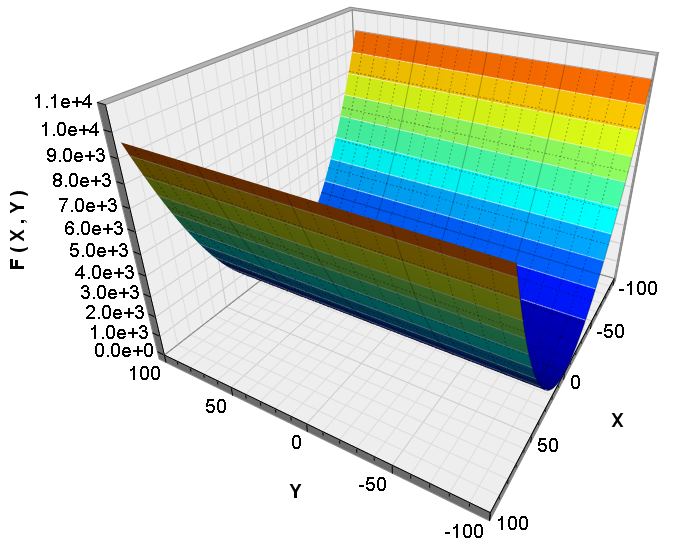
\includegraphics[scale=0.35]{graphics/Elliptic_3d.png}\label{fig:CEC_Elliptic_3d}}
    \hspace{1mm}
    \subfigure[]{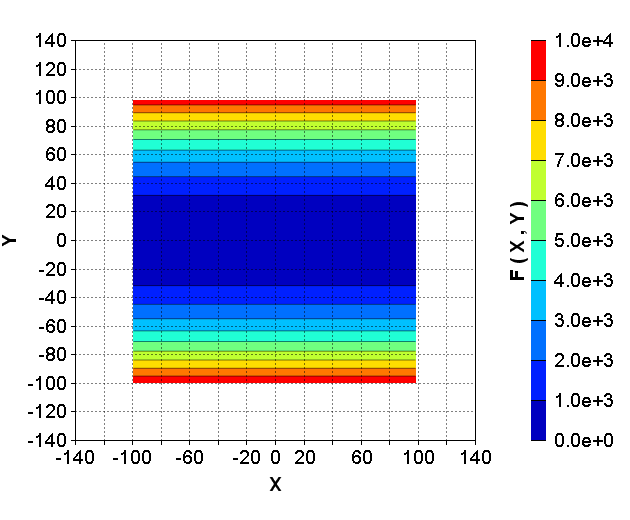
\includegraphics[scale=0.35]{graphics/Elliptic_cont.png}\label{fig:CEC_Elliptic_cont}}
    \caption{Illustration of Elliptic function: (a) Surface and (b) Contour.}
    \label{fig:CEC_Elliptic}
    \end{figure}

    To make this function be nonseparable, an orthogonal matrix will be used to rotate the coordinates. The rotated Elliptic function is defined according to Equation \ref{eq:CEC_Elliptic_rot}.
    \begin{equation}\label{eq:CEC_Elliptic_rot}
    F_{Rot\_Elliptic}(\vec{x}) = F_{Elliptic}(\vec{z}),\ \ \vec{z} = \vec{x} \ast \vec{M},
    \end{equation}
    in which $\vec{M}$ is a $D \times D$ orthogonal matrix, and $\vec{x} = (x_1, x_2, \ldots, x_D)$ is a $D$-dimensional row vector (i.e., a $1 \times D$ matrix).

  \item Schwefel's Problem 1.2: is a naturally nonseparable, which is defined according to Equation (\ref{eq:CEC_Schwefel}). Figure \ref{fig:CEC_Schwefel12} illustrates Schwefel's Problem 1.2.
     \begin{equation}\label{eq:CEC_Schwefel}
     F_{Schwefel}(\vec{x}) = \sum_{i=1}^{D}\Bigl(\sum_{j=1}^{i}x_i\Bigr)^2,
     \end{equation}
      in which $D$ is the number of dimensions and $\vec{x} = (x_1, x_2, \ldots, x_D)$ is a $D$-dimensional row vector (i.e., a $1 \times D$ matrix).
     \begin{figure}[!h]
     \centering
     \subfigure[]{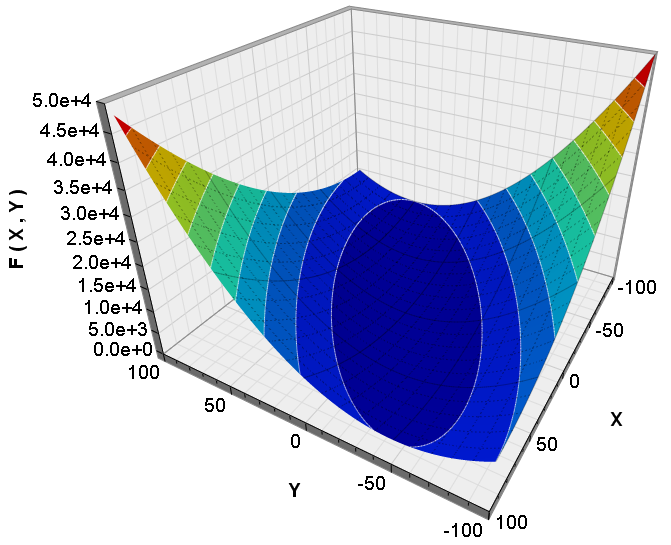
\includegraphics[scale=0.35]{graphics/Schwefel12_3d.png}\label{fig:CEC_Schwefel12_3d}}
     \hspace{1mm}
     \subfigure[]{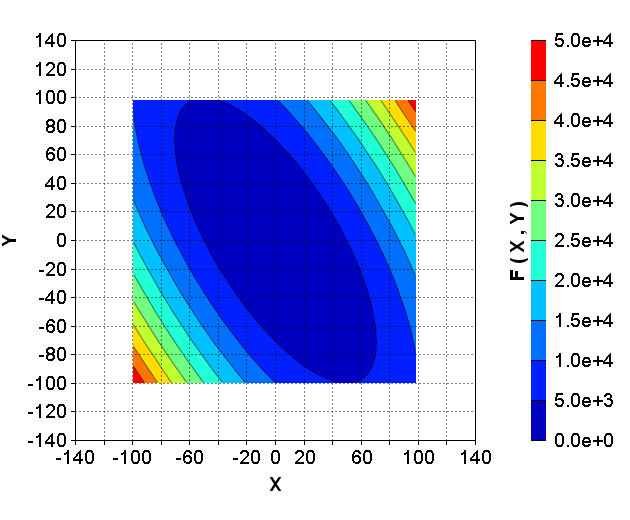
\includegraphics[scale=0.35]{graphics/Schwefel12_cont.png}\label{fig:CEC_Sphere_cont}}
     \caption{Illustration of Schwefel's Problem 1.2: (a) Surface and (b) Contour.}
     \label{fig:CEC_Schwefel12}
     \end{figure}

  \item Rosenbrock's Function: Figure \ref{fig:CEC_Rosenbrock} presents an illustration of Rosenbrock's function, that is also naturally nonseparable and is defined according to Equation (\ref{eq:CEC_Rosenbrock}).
      \begin{equation}\label{eq:CEC_Rosenbrock}
      F_{Rosenbrock}(\vec{x}) = \sum_{i=1}^{D-1}[100(x_i^2 - x_{i+1})^2 + (x_i - 1)^2],
      \end{equation}
      in which $D \geq 2$ is the number of dimensions and $\vec{x} = (x_1, x_2, \ldots, x_D)$ is a $D$-dimensional row vector (i.e., a $1 \times D$ matrix).
      \begin{figure}[!h]
      \centering
      \subfigure[]{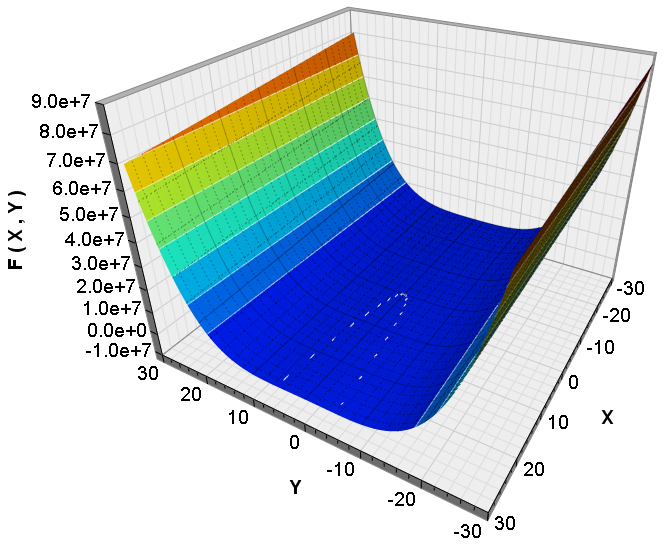
\includegraphics[scale=0.35]{graphics/Rosenbrock_3d.png}\label{fig:CEC_Rosenbrock_3d}}
      \hspace{1mm}
      \subfigure[]{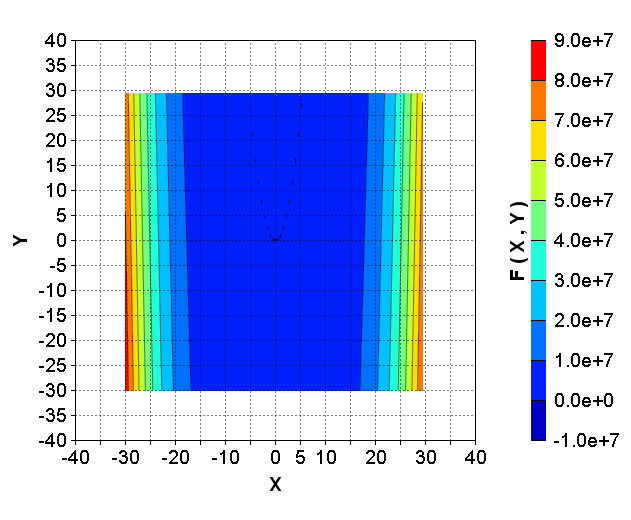
\includegraphics[scale=0.35]{graphics/Rosenbrock_cont.png}\label{fig:CEC_Rosenbrock_cont}}
      \caption{Illustration of Rosenbrock's function: (a) Surface and (b) Contour.}
      \label{fig:CEC_Rosenbrock}
      \end{figure}

  \item The Rotated Rastrigin's Function: The original Rastrigin's function, that can be visualized in Figure \ref{fig:CEC_Rastrigin}, is separable, and is defined according to Equation (\ref{eq:CEC_Rastrigin}).
      \begin{equation}\label{eq:CEC_Rastrigin}
      F_{Rastrigin}(\vec{x}) = \sum_{i=1}^{D}[x_i^2 - 10cos(2 \pi x_i) + 10],
      \end{equation}
      in which $D$ is the number of dimensions and $\vec{x} = (x_1, x_2, \ldots, x_D)$ is a $D$-dimensional row vector (i.e., a $1 \times D$ matrix).
      \begin{figure}[!h]
      \centering
      \subfigure[]{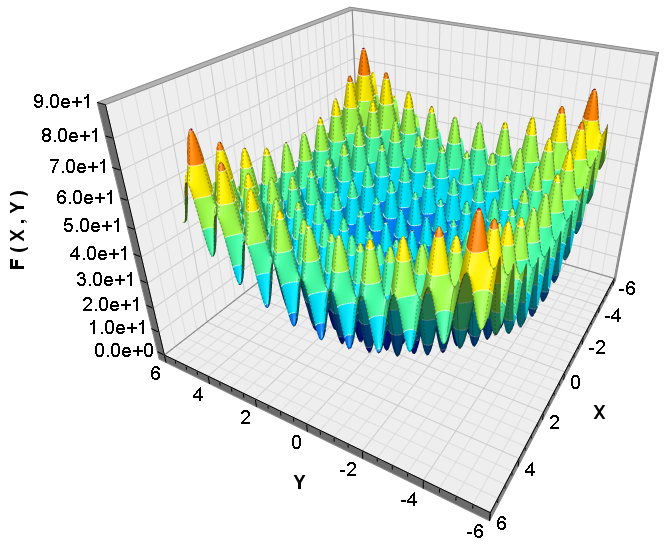
\includegraphics[scale=0.35]{graphics/Rastrigin_3d.png}\label{fig:CEC_Rastrigin_3d}}
      \hspace{1mm}
      \subfigure[]{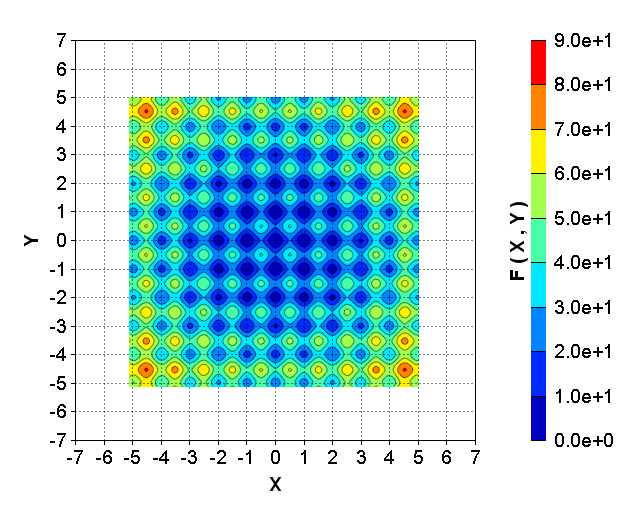
\includegraphics[scale=0.35]{graphics/Rastrigin_cont.png}\label{fig:CEC_Rastrigin_cont}}
      \caption{Illustration of Rastrigin's function: (a) Surface and (b) Contour.}
      \label{fig:CEC_Rastrigin}
      \end{figure}
      Similarly, to make it nonseparable, an orthogonal matrix is also used for coordinate rotation. The Rotated Rasntrigin's function is defined according to Equation (\ref{eq:CEC_Rastrigin_Rot}).
      \begin{equation}\label{eq:CEC_Rastrigin_Rot}
      F_{Rot\_Rastrigin}(\vec{x}) = F_{Rastrigin}(\vec{z}), \ \ \vec{z} = \vec{x} \ast \vec{M},
      \end{equation}
      in which $\vec{M}$ is a $D \times D$ orthogonal matrix, and $\vec{x} = (x_1, x_2, \ldots, x_D)$ is a $D$-dimensional row vector (i.e., a $1 \times D$ matrix). Rastrigin's function is a classical multimodal problem. It is difficult since the number of local optima grows exponentially with the increase of dimensionality.

  \item The Rotated Ackley's Function: The original Ackley's function is separable, and is defined according to Equation (\ref{eq:CEC_Ackley}) and the graphic is illustrated in Figure \ref{fig:CEC_Ackley}.
      \begin{equation}\label{eq:CEC_Ackley}
      F_{Ackley}(\vec{x}) = -20exp\Biggl(-0.2\sqrt{\frac{1}{D}\sum_{i=1}^{D}x_i^2}\Biggr) - exp\Biggl(\frac{1}{D}\sum_{i=1}^{D}cos(2 \pi x_i)\Biggr) + 20 + e,
      \end{equation}
      in which $D$ is the number of dimensions and $\vec{x} = (x_1, x_2, \ldots, x_D)$ is a $D$-dimensional row vector (i.e., a $1 \times D$ matrix).
      \begin{figure}[!h]
      \centering
      \subfigure[]{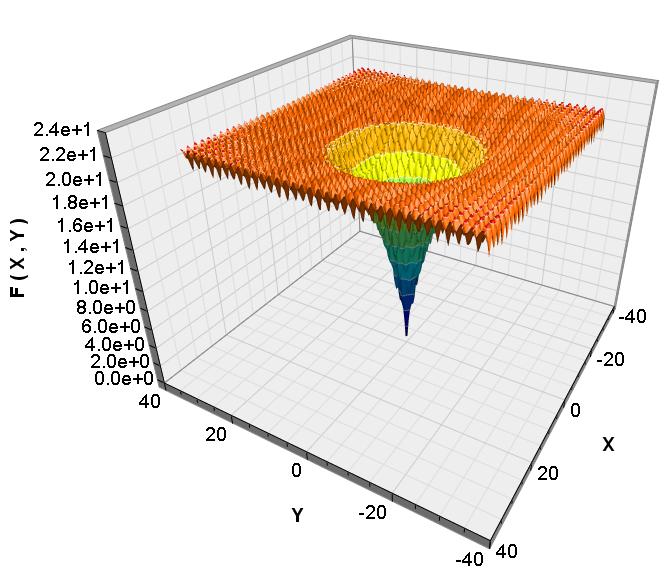
\includegraphics[scale=0.35]{graphics/Ackley_3d.png}\label{fig:CEC_Ackley_3d}}
      \hspace{1mm}
      \subfigure[]{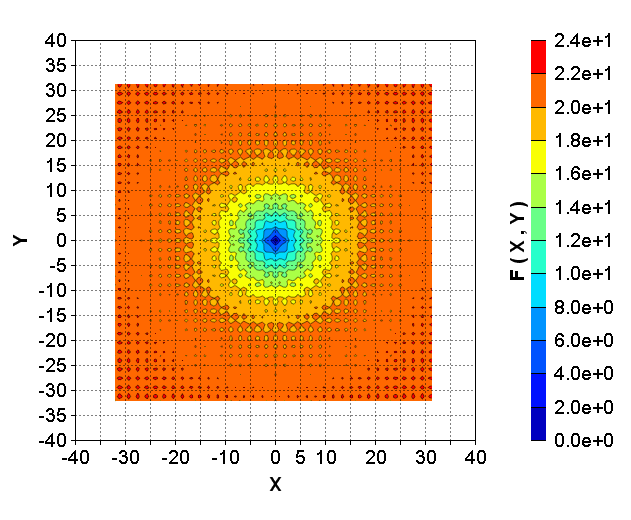
\includegraphics[scale=0.35]{graphics/Ackley_cont.png}\label{fig:CEC_Ackley_cont}}
      \caption{Illustration of Ackley's function: (a) Surface and (b) Contour.}
      \label{fig:CEC_Ackley}
      \end{figure}
      To make it nonseparable, an orthogonal matrix is used again for coordinate rotation. The Rotated Ackley's function is defined according to Equation (\ref{eq:CEC_Ackley_Rot}).
      \begin{equation}\label{eq:CEC_Ackley_Rot}
      F_{Rot\_Ackley}(\vec{x}) = F_{Ackley}(\vec{z}), \ \ \vec{z} = \vec{x} \ast \vec{M},
      \end{equation}
      in which $\vec{M}$ is a $D \times D$ orthogonal matrix, and $\vec{x} = (x_1, x_2, \ldots, x_D)$ is a $D$-dimensional row vector (i.e., a $1 \times D$ matrix).
\end{itemize}

The benchmark functions are listed according to the separability degree of variables. The following, we describe the mathematical formulas and properties of these functions.

\subsection{Separable Functions}
In this subsection, the variables are: (\emph{i}) $D = 1000$ is the number of dimensions; (\emph{ii}) $\vec{x} = (x_1, x_2, \ldots, x_D)$ is the candidate solution; and (\emph{iii}) $\vec{z} = (z_1, z_2, \ldots, z_D)$ is the shifted candidate solution, where $\vec{z} = \vec{x} - \vec{o}$, $\vec{o} = (o_1, o_2, \ldots, o_D)$ is the (shifted global optimum). The functions of this group are listed as follows.
  \begin{itemize}
    \item $F1$ - Shifted Elliptic Function: the Shifted Elliptic function is unimodal, separable, scalable and its formula is defined according to Equation (\ref{eq:CEC_F1}).
        \begin{equation}\label{eq:CEC_F1}
            F_1(\vec{x}) = F_{Elliptic}(\vec{z}) = \sum_{i=1}^{D}(10^6)^{\frac{i-1}{D-1}}z_i^2;
        \end{equation}
    \item $F2$ - Shifted Rastrigin's Function: the Shifted Rastrigin's function is multimodal, separable, scalable and its formula is defined according to Equation (\ref{eq:CEC_F2}).
        \begin{equation}\label{eq:CEC_F2}
            F_2(\vec{x}) = F_{Rastrigin}(\vec{z}) = \sum_{i=1}^{D}[z_i^2 - 10cos(2 \pi z_i) + 10];
        \end{equation}    
    \item  $F3$ - Shifted Ackley's Function: the Shifted Ackley's function is multimodal, separable, scalable and its formula is defined according to Equation (\ref{eq:CEC_F3}).
        \begin{equation}\label{eq:CEC_F3}
            F_3(\vec{x}) = F_{Ackley}(\vec{z}) = -20exp\Biggl(-0.2 \sqrt{\frac{1}{D}\sum_{i=1}^{D}z_i^2}\Biggr) - exp\Biggl(\frac{1}{D}\sum_{i=1}^{D}cos(2 \pi z_i)\Biggr) + 20 + e.
        \end{equation}
  \end{itemize}
     
\subsection{Single-group $m$-nonseparable Functions}
In this subsection, the variables are: (\emph{i}) $D = 1000$ is the number of dimensions; (\emph{ii}) $m = 50$ is group size, (\emph{iii}) $P$ is a random permutation of ${1, 2, \ldots, D}$; (\emph{iv}) $\vec{x} = (x_1, x_2, \ldots, x_D)$ is the candidate solution; and  (\emph{v}) $\vec{z} = (z_1, z_2, \ldots, z_D)$ is the shifted candidate solution, where $\vec{z} = \vec{x} - \vec{o}$, $\vec{o} = (o_1, o_2, \ldots, o_D)$ is the (shifted global optimum). The functions of this group are listed as follows.
 \begin{itemize}
   \item $F4$ - Single-group Shifted and $m$-rotated Elliptic Function: the Single-group Shifted and $m$-rotated Elliptic function is unimodal, has single-group with $m$ rotated and nonseparable variables, and its formula is defined according to Equation (\ref{eq:CEC_F4}).
        \begin{equation}\label{eq:CEC_F4}
            F_4(\vec{x}) = F_{Rot\_{Elliptic}}[\vec{z}(P_1:P_m)] \ast 10^6 + F_{Elliptic}[\vec{z}(P_{m+1}:P_D)],
        \end{equation}
   \item $F5$ - Single-group Shifted and $m$-rotated Rastrigin's Function: the Single-group Shifted and $m$-rotated Rastrigin's function is multimodal, has single-group with $m$ rotated and nonseparable variables, and its formula is defined according to Equation (\ref{eq:CEC_F5}).
        \begin{equation}\label{eq:CEC_F5}
            F_5(\vec{x}) = F_{Rot\_{Rastrigin}}[\vec{z}(P_1:P_m)] \ast 10^6 + F_{Rastrigin}[\vec{z}(P_{m+1}:P_D)],
        \end{equation}

   \item $F6$ - Single-group Shifted and $m$-rotated Ackley's Function: the Single-group Shifted and $m$-rotated Ackley's function is multimodal, has single-group with $m$ rotated and nonseparable variables, and its formula is defined according to Equation (\ref{eq:CEC_F6}).
        \begin{equation}\label{eq:CEC_F6}
            F_6(\vec{x}) = F_{Rot\_{Ackley}}[\vec{z}(P_1:P_m)] \ast 10^6 + F_{Ackley}[\vec{z}(P_{m+1}:P_D)],
        \end{equation}

   \item $F7$ - Single-group Shifted and $m$-dimensional Schwefel's Problem 1.2: the Single-group Shifted and $m$-dimensional Schwefel's Problem 1.2 is unimodal, has single-group with $m$ nonseparable variables, and its formula is defined according to Equation (\ref{eq:CEC_F7}).
        \begin{equation}\label{eq:CEC_F7}
            F_7(\vec{x}) = F_{Schwefel}[\vec{z}(P_1:P_m)] \ast 10^6 + F_{Sphere}[\vec{z}(P_{m+1}:P_D)],
        \end{equation}

   \item $F8$ - Single-group Shifted and $m$-dimensional Rosenbrock's Function: The Single-group Shifted and $m$-dimensional Rosenbrock's function is multimodal, has single-group with $m$ nonseparable variables, and its formula is defined according to Equation (\ref{eq:CEC_F8}).
        \begin{equation}\label{eq:CEC_F8}
            F_8(\vec{x}) = F_{Rosenbrock}[\vec{z}(P_1:P_m)] \ast 10^6 + F_{Sphere}[\vec{z}(P_{m+1}:P_D)],
        \end{equation}
 \end{itemize}
     
\subsection{$D/2m$-group $m$-nonseparable Functions}
In this subsection, the variables are: (\emph{i}) $D = 1000$ is the number of dimensions; (\emph{ii}) $m = 50$ is group size; (\emph{iii}) $P$ is a random permutation of ${1, 2, \ldots, D}$, (\emph{iv}) (\emph{iv})$\vec{x} = (x_1, x_2, \ldots, x_D)$ is the candidate solution; and (\emph{v}) $\vec{z} = (z_1, z_2, \ldots, z_D)$ is the shifted candidate solution, where $\vec{z} = \vec{x} - \vec{o}$, $\vec{o} = (o_1, o_2, \ldots, o_D)$ is the (shifted global optimum). The functions of this group are listed as follows.

\begin{itemize}
  \item $F9$ - $D/2m$-group Shifted and $m$-rotated Elliptic Function: The $D/2m$-group Shifted and $m$-rotated Elliptic function is unimodal, has $D/2m$-group with $m$ rotated and nonseparable variables, and its formula is defined according to Equation (\ref{eq:CEC_F9}).
      \begin{equation}\label{eq:CEC_F9}
            F_9(\vec{x}) = \sum_{k=1}^{\frac{D}{2m}}F_{Rot\_{Elliptic}}[\vec{z}(P_{(k-1) \ast m+1}:P_{k \ast m})] + F_{Elliptic}[\vec{z}(P_{\frac{D}{2}+1}:P_D)],
      \end{equation}
  \item $F10$ - $D/2m$-group Shifted and $m$-rotated Rastrigin's Function: The $D/2m$-group Shifted and $m$-rotated Rastrigin's function is multimodal, has $D/2m$-group with $m$ rotated and nonseparable variables, and its formula is defined according to Equation (\ref{eq:CEC_F10}).
      \begin{equation}\label{eq:CEC_F10}
            F_{10}(\vec{x}) = \sum_{k=1}^{\frac{D}{2m}}F_{Rot\_{Rastrigin}}[\vec{z}(P_{(k-1) \ast m+1}:P_{k \ast m})] + F_{Rastrigin}[\vec{z}(P_{\frac{D}{2}+1}:P_D)],
      \end{equation}
  \item $F11$ - $D/2m$-group Shifted and $m$-rotated Ackley's Function: The $D/2m$-group Shifted and $m$-rotated Ackley's function is multimodal, has $D/2m$-group with $m$ rotated and nonseparable variables, and its formula is defined according to Equation (\ref{eq:CEC_F11}).
      \begin{equation}\label{eq:CEC_F11}
            F_{11}(\vec{x}) = \sum_{k=1}^{\frac{D}{2m}}F_{Rot\_{Ackley}}[\vec{z}(P_{(k-1) \ast m+1}:P_{k \ast m})] + F_{Ackley}[\vec{z}(P_{\frac{D}{2}+1}:P_D)],
      \end{equation}
  \item $F12$ - $D/2m$-group Shifted and $m$-dimensional Schwefel's Problem 1.2: The $D/2m$-group Shifted and $m$-dimensional Schwefel's Problem 1.2 is unimodal, has $D/2m$-group with $m$ nonseparable variables, and its formula is defined according to Equation (\ref{eq:CEC_F12}).
      \begin{equation}\label{eq:CEC_F12}
            F_{12}(\vec{x}) = \sum_{k=1}^{\frac{D}{2m}}F_{Schwefel}[\vec{z}(P_{(k-1) \ast m+1}:P_{k \ast m})] + F_{Sphere}[\vec{z}(P_{\frac{D}{2}+1}:P_D)],
      \end{equation}
  \item $F13$ - $D/2m$-group Shifted and $m$-dimensional Rosenbrock's Function: The $D/2m$-group Shifted and $m$-dimensional Rosenbrock's function is multimodal, has $D/2m$-group with $m$ nonseparable variables, and its formula is defined according to Equation (\ref{eq:CEC_F13}).
      \begin{equation}\label{eq:CEC_F13}
            F_{13}(\vec{x}) = \sum_{k=1}^{\frac{D}{2m}}F_{Rosenbrock}[\vec{z}(P_{(k-1) \ast m+1}:P_{k \ast m})] + F_{Sphere}[\vec{z}(P_{\frac{D}{2}+1}:P_D)],
      \end{equation}
\end{itemize}

\subsection{$D/m$-group $m$-nonseparable Functions}
In this subsection, the variables are: (\emph{i}) $D = 1000$ is the number of dimensions; (\emph{ii}) $m = 50$ is group size; (\emph{iii}) $P$ is a random permutation of ${1, 2, \ldots, D}$; (\emph{iv}) $\vec{x} = (x_1, x_2, \ldots, x_D)$ is the candidate solution; and (\emph{v}) $\vec{z} = (z_1, z_2, \ldots, z_D)$ is the shifted candidate solution, where $\vec{z} = \vec{x} - \vec{o}$, $\vec{o} = (o_1, o_2, \ldots, o_D)$ is the (shifted global optimum). The functions of this group are listed as follows.

\begin{itemize}
  \item $F14$ - $D/m$-group Shifted and $m$-rotated Elliptic Function: The $D/m$-group Shifted and $m$-rotated Elliptic function is unimodal, has $D/2m$-group with $m$ rotated and nonseparable variables, and its formula is defined according to Equation (\ref{eq:CEC_F14}).
      \begin{equation}\label{eq:CEC_F14}
            F_{14}(\vec{x}) = \sum_{k=1}^{\frac{D}{m}}F_{Rot\_{Elliptic}}[\vec{z}(P_{(k-1) \ast m+1}:P_{k \ast m})],
      \end{equation}
  \item $F15$ - $D/m$-group Shifted and $m$-rotated Rastrigin's Function: The $D/m$-group Shifted and $m$-rotated Rastrigin's function is multimodal, has $D/m$-group with $m$ rotated and nonseparable variables, and its formula is defined according to Equation (\ref{eq:CEC_F15}).
      \begin{equation}\label{eq:CEC_F15}
            F_{15}(\vec{x}) = \sum_{k=1}^{\frac{D}{m}}F_{Rot\_{Rastrigin}}[\vec{z}(P_{(k-1) \ast m+1}:P_{k \ast m})],
      \end{equation}
  \item $F16$ - $D/m$-group Shifted and $m$-rotated Ackley's Function: The $D/m$-group Shifted and $m$-rotated Ackley's function is multimodal, has $D/m$-group with $m$ rotated and nonseparable variables, and its formula is defined according to Equation (\ref{eq:CEC_F16}).
      \begin{equation}\label{eq:CEC_F16}
            F_{16}(\vec{x}) = \sum_{k=1}^{\frac{D}{m}}F_{Rot\_{Ackley}}[\vec{z}(P_{(k-1) \ast m+1}:P_{k \ast m})],
      \end{equation}
  \item $F17$ - $D/m$-group Shifted and $m$-dimensional Schwefel's Problem 1.2: The $D/m$-group Shifted and $m$-dimensional Schwefel's Problem 1.2 is unimodal, has $D/m$-group with $m$ nonseparable variables, and its formula is defined according to Equation (\ref{eq:CEC_F17}).
      \begin{equation}\label{eq:CEC_F17}
      F_{17}(\vec{x}) = \sum_{k=1}^{\frac{D}{m}}F_{Schwefel}[\vec{z}(P_{(k-1) \ast m+1}:P_{k \ast m})];
      \end{equation}
  \item $F18$ - $D/m$-group Shifted and $m$-dimensional Rosenbrock's Function: The $D/m$-group Shifted and $m$-dimensional Rosenbrock's function is multimodal, has $D/m$-group with $m$ nonseparable variables, and its formula is defined according to Equation (\ref{eq:CEC_F18}).
      \begin{equation}\label{eq:CEC_F18}
      F_{18}(\vec{x}) = \sum_{k=1}^{\frac{D}{m}}F_{Rosenbrock}[\vec{z}(P_{(k-1) \ast m+1}:P_{k \ast m})].
      \end{equation}
\end{itemize}

\subsection{Nonseparable Functions}
In this subsection, the variables are: (\emph{i}) $D = 1000$ is the number of dimensions; (\emph{ii}) $\vec{x} = (x_1, x_2, \ldots, x_D)$ is the candidate solution; and (\emph{iii}) $\vec{z} = (z_1, z_2, \ldots, z_D)$ is the shifted candidate solution, where $\vec{z} = \vec{x} - \vec{o}$, $\vec{o} = (o_1, o_2, \ldots, o_D)$ is the (shifted global optimum). The functions of this group are listed as follows.

\begin{itemize}
  \item $F19$ - Shifted Schwefel's Problem 1.2: The Shifted Schwefel's Problem 1.2 is unimodal, fully-nonseparable and its formula is defined according to Equation (\ref{eq:CEC_F19}).
      \begin{equation}\label{eq:CEC_F19}
      F_{19}(\vec{x}) = F_{Schwefel}(\vec{z})\sum_{i=1}^{n}\Biggl(\sum_{j=1}^{i}x_i \Biggr)^2;
      \end{equation}
  \item $F20$ - Shifted Rosenbrock's Function: The Shifted Rosenbrock's function is multimodal, fully-nonseparable and its formula is defined according to Equation (\ref{eq:CEC_F20}).
      \begin{equation}\label{eq:CEC_F20}
      F_{20}(\vec{x}) = F_{Rosenbrock}(\vec{z}) = \sum_{i=1}^{D-1}[100(z_i^2 - z_{i+1})^2 + (z_i - 1)^2].
      \end{equation}
\end{itemize}
    
\subsection{Definition of Search Space Boundaries and Global Optimum}
The Table \ref{tab:SearchSpace_Optimum} presents the search space boundaries and global optimum of each benchmark function. As observed, these functions are minimization problems.
\begin{table}[!h]
\caption{Benchmark functions, search space boundaries and global optimum position.}
\centering
\begin{tabular}{c c c}
\hline
Function  &   Search Space               &  Global Optimum  \\
\hline
$F1$    & $-100 \leq x_i \leq 100$     & $0.0^D$ \\
$F2$    & $-5 \leq x_i \leq 5$     & $0.0^D$ \\
$F3$    & $-32 \leq x_i \leq 32$     & $0.0^D$ \\
$F4$    & $-100 \leq x_i \leq 100$     & $0.0^D$ \\
$F5$    & $-5 \leq x_i \leq 5$     & $0.0^D$ \\
$F6$    & $-32 \leq x_i \leq 32$     & $0.0^D$ \\
$F7$    & $-100 \leq x_i \leq 100$     & $0.0^D$ \\
$F8$    & $-100 \leq x_i \leq 100$     & $0.0^D$ \\
$F9$    & $-100 \leq x_i \leq 100$     & $0.0^D$ \\
$F10$    & $-5 \leq x_i \leq 5$     & $0.0^D$ \\
$F11$    & $-32 \leq x_i \leq 32$     & $0.0^D$ \\
$F12$    & $-100 \leq x_i \leq 100$     & $0.0^D$ \\
$F13$    & $-100 \leq x_i \leq 100$     & $0.0^D$ \\
$F14$    & $-100 \leq x_i \leq 100$     & $0.0^D$ \\
$F15$    & $-5 \leq x_i \leq 5$     & $0.0^D$ \\
$F16$    & $-32 \leq x_i \leq 32$     & $0.0^D$ \\
$F17$    & $-100 \leq x_i \leq 100$     & $0.0^D$ \\
$F18$    & $-100 \leq x_i \leq 100$     & $0.0^D$ \\
$F19$    & $-100 \leq x_i \leq 100$     & $0.0^D$ \\
$F20$    & $-100 \leq x_i \leq 100$     & $0.0^D$ \\
\hline
\end{tabular}
\label{tab:SearchSpace_Optimum}
\end{table}

\section{Experimental Methodology}
This section presents the strategies adopted in the realization the experiments showed in this dissertation. The topics of this section are: environment of simulation, in which the framework used to realized the experiments is described, evaluation metrics used to assess the performance of the algorithms, and the simulation setup, in which the values of the parameters are presented.

\subsection{Environment of the Simulations}
All simulations were realized in a framework, called \emph{Dynamic Optimization System Simulator} (DOSS) proposed by Carneiro \cite{DOSS:Castro2010}. This framework presents a suitable infrastructure to develop and simulate the algorithms. It was developed using the Java programming language \cite{DOSS:Java2005}, the Eclipse tool \cite{DOSS:Eclipse2011} and also Maven tool \cite{DOSS:Maven2011}. In the Eclipse tool, we can write the source code and the Maven tool is used to manage the dependencies and compile the projects. The framework has the graphical user interface (GUI), called \emph{Dynamic Optimization System Analyzer} (DOSA). This interface allows one to create test scenarios and evaluate the simulations results \cite{DOSS:Castro2010}.

Figure \ref{fig:DOSA-DOSS} illustrates the main screen of DOSA, in which the test scenarios are build selecting: the algorithm, the optimization problem, the evaluation metric, and the stopping criteria. Then, one can define the configuration of the experiment, assigning values for the parameters of the algorithm, the number of dimensions of the problem, the stop condition and the number of trials.

\begin{figure}[!h]
\centering
 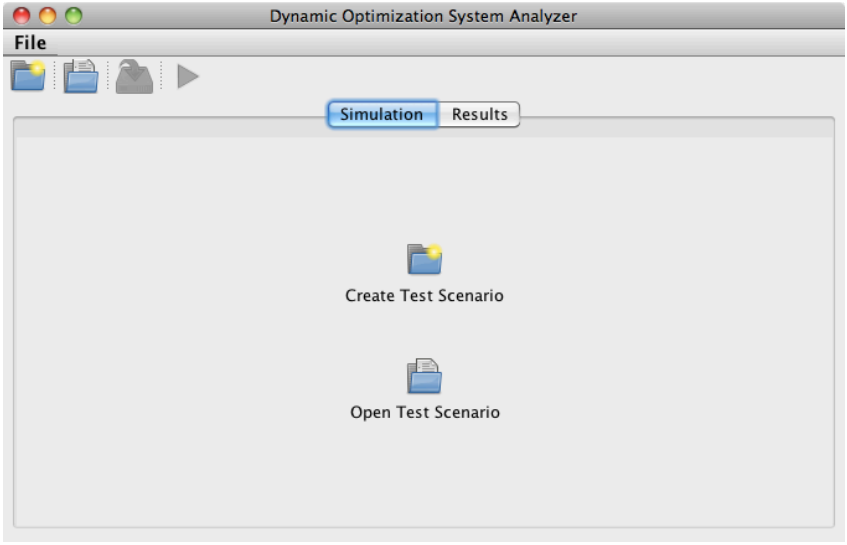
\includegraphics[width=0.65\textwidth]{image/DOSA-DOSS.png}
 \caption{\small{Illustration of the DOSA main screen.}}
 \label{fig:DOSA-DOSS}
\end{figure}

We used the software called OriginPro version 8.6 to build the graphics \cite{DOSS:Origin2011} of generated results. OriginPro is proprietary software very used to generate interactive scientific graphing and data analysis.

\subsection{Metrics of Evaluation}
The evaluation metrics used to compare the performance of the algorithms are: the convergence velocity, it measures how fast the algorithm converges; the scalability, it estimates the degradation of the performance as the complexity of the problem (number of dimensions) increases; and the average value for the fitness at the end of each trial.
We also performed statistical tests when the difference between the results of the algorithms assessing the boxplots is not too large. We used the Wilcoxon non-parametric test \cite{Wil:Lowry2011}. %This evaluation is a complement of other evaluations, to guarantee the reliability of results.


\subsection{Experiments Setup}
In all experiments, we used 30 particles to ABeePSO, APSO and PSO and 60 bees to ABC. We used a double of bees in ABC because just a half are food sources and we would like to assess the same number of potential solutions. We used 6 clans for the algorithms ClanPSO, ClanAPSO and ClanABeePSO, \textit{i.e.} the populations of these algorithms are composed by 6 clans of 5 particles. We used the local communication topology for the ABeePSO, APSO and PSO algorithm. The stagnation counter ($MaxTrial$) of ABC algorithm is equal to 5.

We used the number of dimensions equal to 100, 300, 500 or 1,000 dimensions. The number of iterations depends on the number of dimensions, we performed 1,000, 3,000, 5,000 and 10,000 iterations, respectively. The stop criterion for these algorithms is the number of iterations. This condition was chosen because it limits the number of fitness evaluations and allows a fair comparison between the algorithms.

\begin{table}[!h]
\caption{\small{The number of parameters of each algorithm.}}
\centering
\begin{tabular}{>{\centering\arraybackslash}m{1in} | >{\centering\arraybackslash}m{1in} | >{\centering\arraybackslash}m{2in}}
\hline
\textbf{Algorithm}  & \textbf{Number of Parameters} & \textbf{Parameters}\\
\hline
\textbf{PSO}      &   5  & $N$, $c_1$, $c_2$, $\omega_{min}$, $\omega_{max}$\\
\textbf{APSO}     &   5  & $N$, $c_1$, $c_2$, $\omega_{min}$, $\omega_{max}$\\
\textbf{ClanPSO}  &   6  & $N$, $c_1$, $c_2$, $\omega_{min}$, $\omega_{max}$, $N_{pc}$\\
\textbf{ClanAPSO} &   6  & $N$, $c_1$, $c_2$, $\omega_{min}$, $\omega_{max}$, $N_{pc}$\\
\textbf{ABC}      &   2  & $2 \cdot SN$, $MaxTrial$\\
\textbf{FSS}      &   6  & $S$, $W_{scale}$, $step_{vol\_initial}$, $step_{vol\_final}$, $step_{ind\_initial}$, $step_{ind\_final}$ \\
\hline
\end{tabular}
\label{tab:Param_Algorithm}
\end{table}


%The range of $step_{ind}$ is 0.01 to 0.5.

\pagebreak
